\documentclass[11pt,letterpaper]{article}

\usepackage[margin=2.2cm]{geometry}
\usepackage{amsmath}
\usepackage{array}
\usepackage{booktabs}
\usepackage{graphicx}
\usepackage{pdflscape}

\title{Memoria de calculo comparada\\Proyecto IE0413}
\author{Daniel Gerardo Madriz Chavarria C24478\\
Fabricio Torres Jimenez C27803\\
Kenneth Daniel Vizcaino Jimenez C09331}
\date{I ciclo 2026}

\begin{document}

\maketitle

\section*{Ruta usada}

Se usa la version minima del sintetizador:

\begin{itemize}
  \item un \texttt{NE555} como oscilador astable para la onda cuadrada;
  \item una etapa RC con transistor de descarga para la sierra positiva;
  \item una senal cuadrada equivalente a \(f_0/2\), cambio de nivel e
  integrador con \texttt{LF353} para la triangular;
  \item un filtro activo Chebyshev de quinto orden con \texttt{LF353}.
\end{itemize}

Esta ruta evita agregar otro oscilador o un bloque digital dedicado para no
complicar los calculos. La comparacion contra LTspice se hace por etapa, ya que
cada bloque tiene una formula directa.

\begin{landscape}
\section*{Esquematico resumido}
\begin{center}
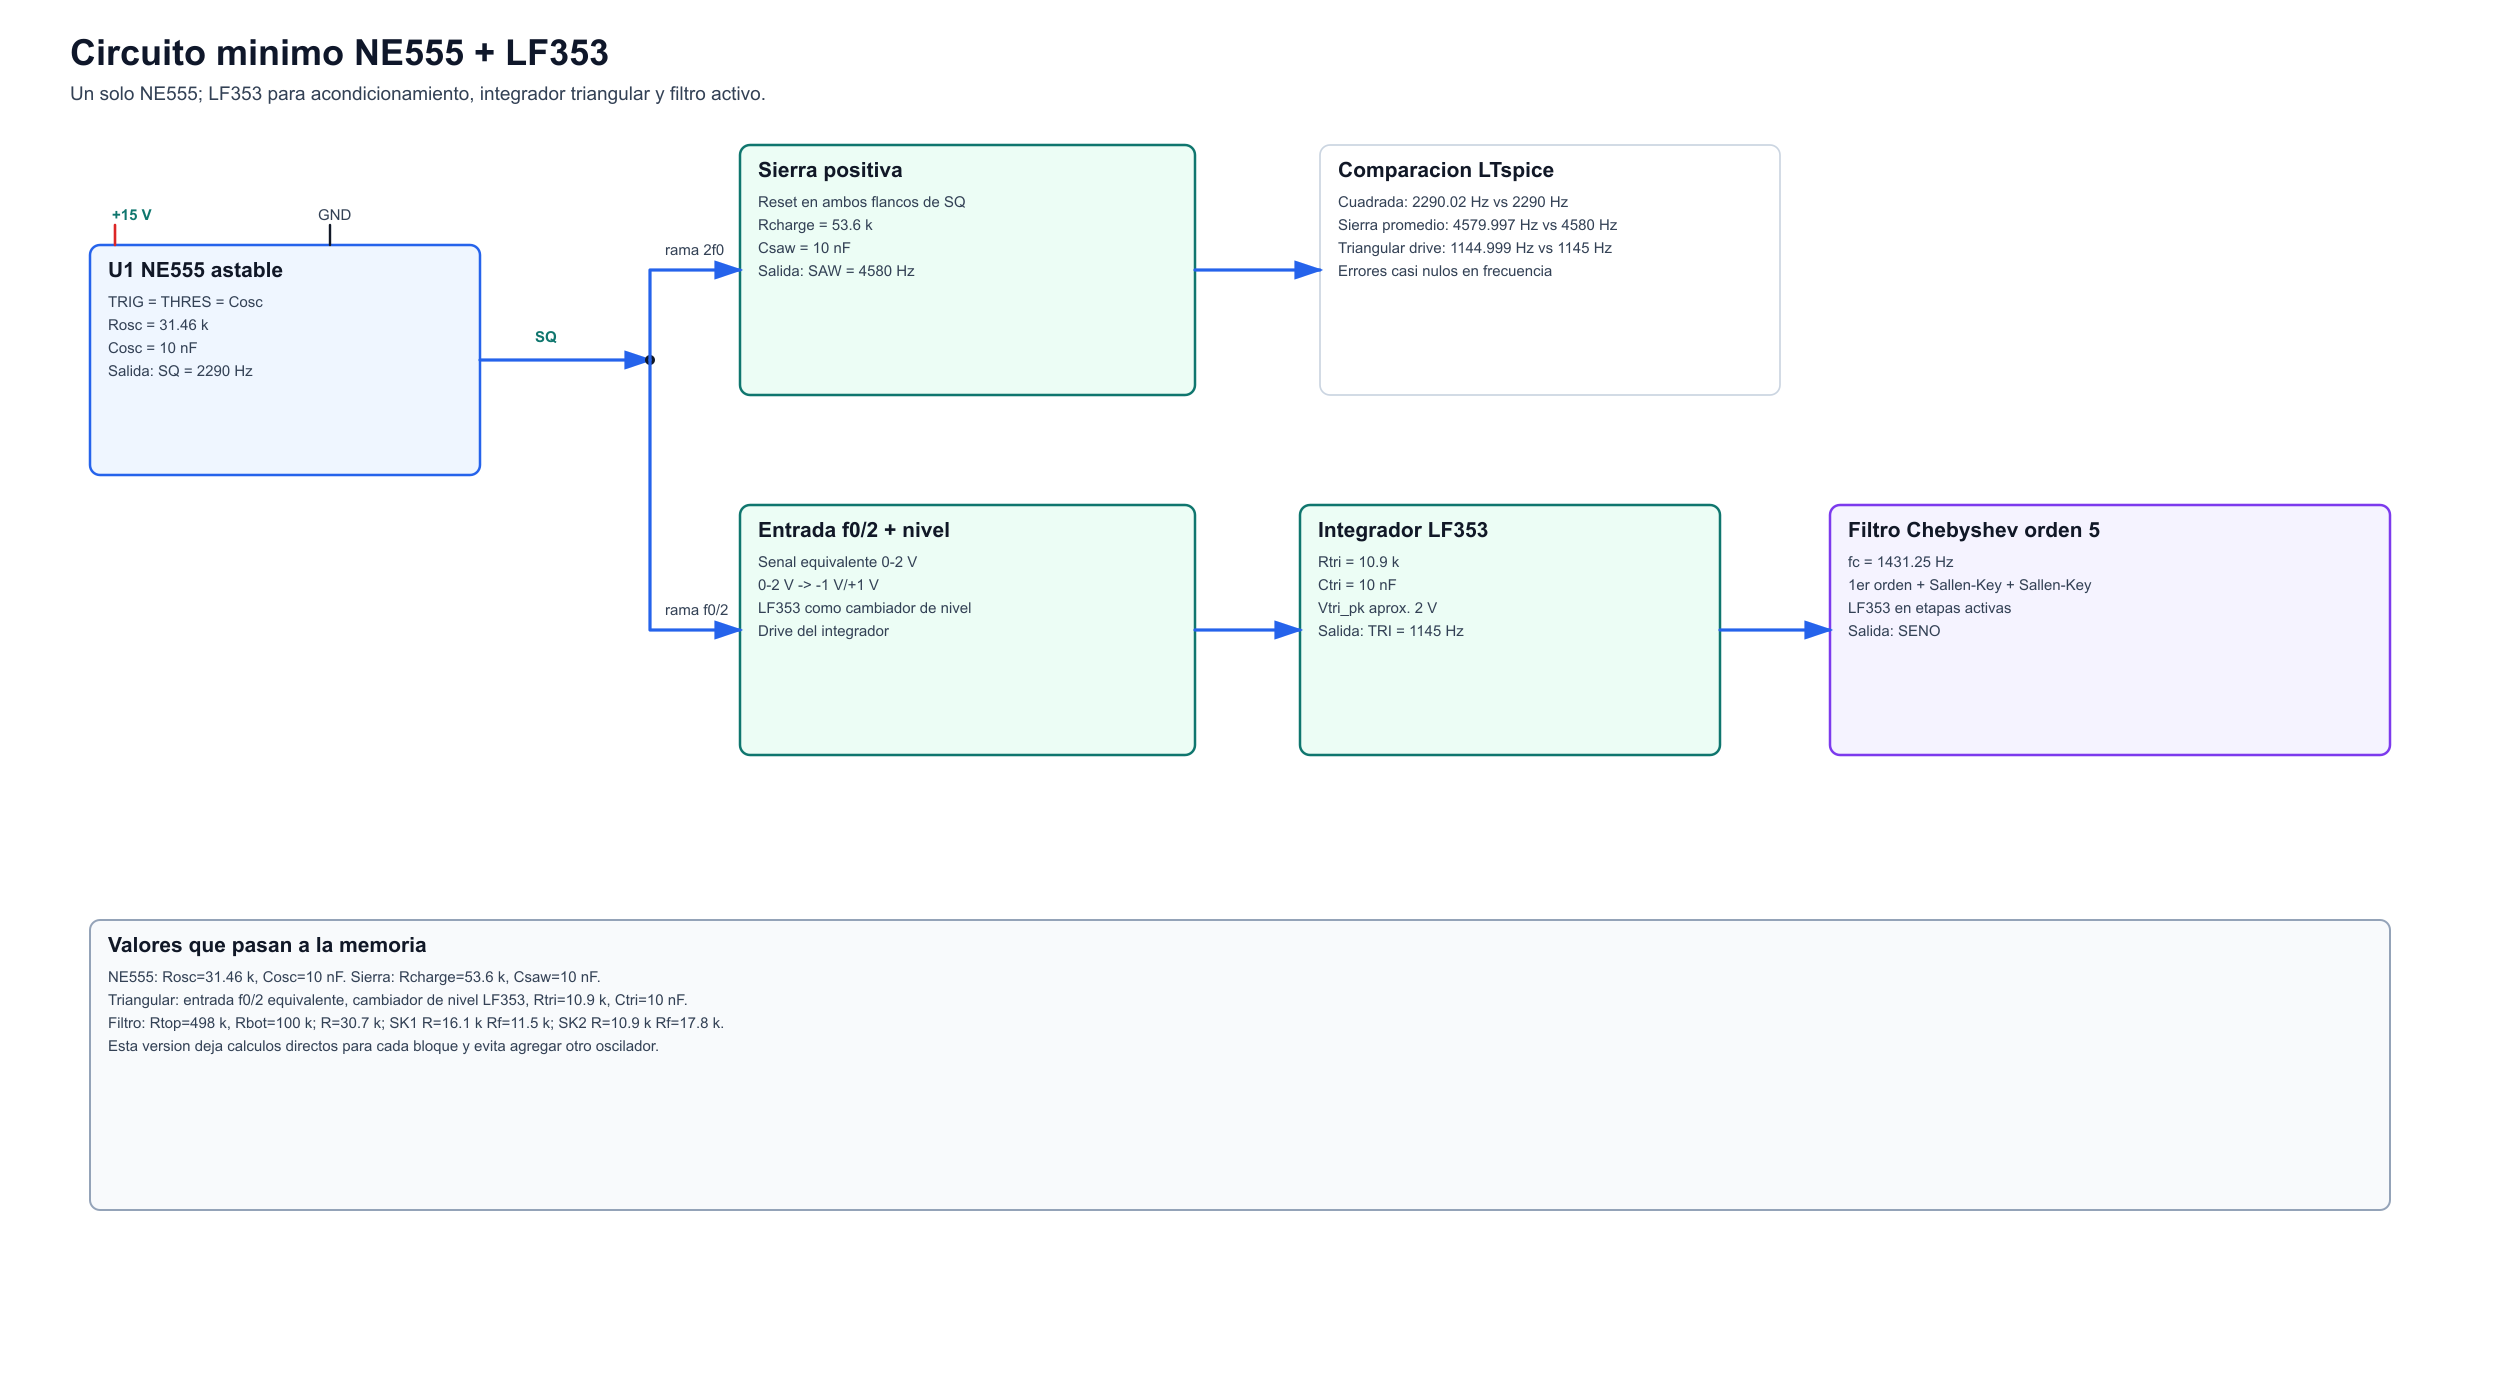
\includegraphics[width=\linewidth,height=0.82\textheight,keepaspectratio]{figuras/esquematico_minimo_ne555_lf353.png}
\end{center}
\end{landscape}

\section{Datos del grupo}

Por el orden alfabetico de apellidos:

\[
X=2, \qquad Y=2, \qquad Z=9.
\]

\[
f_0=\left(X+\frac{Y}{10}+\frac{Z}{100}\right)1000~\text{Hz}.
\]

\[
f_0=\left(2+\frac{2}{10}+\frac{9}{100}\right)1000.
\]

\[
\boxed{f_0=2290~\text{Hz}}.
\]

Las frecuencias pedidas son:

\[
f_{saw}=2f_0=4580~\text{Hz}.
\]

\[
f_{tri}=\frac{f_0}{2}=1145~\text{Hz}.
\]

Como \(Z=9\), la respuesta del filtro es Chebyshev.

\section{Onda cuadrada con NE555}

El \texttt{NE555} se usa como astable tipo Schmitt. El capacitor del oscilador
cambia entre:

\[
V_L=\frac{V_{CC}}{3},
\qquad
V_H=\frac{2V_{CC}}{3}.
\]

Con la misma resistencia para carga y descarga:

\[
t_H=R_{osc}C_{osc}\ln(2),
\qquad
t_L=R_{osc}C_{osc}\ln(2).
\]

\[
T=2R_{osc}C_{osc}\ln(2).
\]

\[
f_0=\frac{1}{2R_{osc}C_{osc}\ln(2)}.
\]

Se despeja:

\[
R_{osc}=\frac{1}{2f_0C_{osc}\ln(2)}.
\]

Con:

\[
C_{osc}=10~\text{nF},
\qquad
f_0=2290~\text{Hz},
\]

\[
R_{osc}=
\frac{1}{2(2290)(10\times10^{-9})\ln(2)}.
\]

\[
R_{osc}=31.55~\text{k}\Omega.
\]

En LTspice se uso:

\[
\boxed{R_{osc}=31.46~\text{k}\Omega}
\]

para compensar ligeramente el modelo del \texttt{NE555}.

\section{Onda diente de sierra}

La sierra se obtiene cargando \(C_{saw}\) desde \(+15~\text{V}\) por medio de
una resistencia y descargandolo rapidamente con un transistor en cada flanco de
la cuadrada. Como se descarga en ambos flancos:

\[
f_{saw}=2f_0.
\]

\[
T_{saw}=\frac{1}{2f_0}.
\]

\[
T_{saw}=\frac{1}{2(2290)}=218.34~\mu\text{s}.
\]

Para la carga RC:

\[
v_C(t)=V_{CC}\left(1-e^{-t/(RC)}\right).
\]

Se desea que:

\[
v_C(T_{saw})=V_{saw,pk}.
\]

Entonces:

\[
V_{saw,pk}=V_{CC}\left(1-e^{-T_{saw}/(R_{charge}C_{saw})}\right).
\]

Despejando:

\[
R_{charge}=
\frac{-T_{saw}}
{C_{saw}\ln\left(1-\frac{V_{saw,pk}}{V_{CC}}\right)}.
\]

Con:

\[
V_{CC}=15~\text{V},
\qquad
V_{saw,pk}=5~\text{V},
\qquad
C_{saw}=10~\text{nF},
\]

\[
R_{charge}=
\frac{-218.34\times10^{-6}}
{(10\times10^{-9})\ln\left(1-\frac{5}{15}\right)}.
\]

\[
R_{charge}=53.85~\text{k}\Omega.
\]

Se usa el valor:

\[
\boxed{R_{charge}=53.6~\text{k}\Omega}.
\]

\section{Onda triangular con LF353}

La senal a \(f_0/2\) se acondiciona a una cuadrada de \(-1~\text{V}\) a
\(+1~\text{V}\). Esta senal entra a un integrador inversor con \texttt{LF353}.

Para el integrador:

\[
\frac{dv_o}{dt}=-\frac{v_i}{R_{tri}C_{tri}}.
\]

Durante medio periodo de la triangular, la entrada tiene magnitud \(V_{drv}\).
El cambio de voltaje es:

\[
\Delta V=\frac{V_{drv}T_0}{R_{tri}C_{tri}}.
\]

La triangular debe cambiar de \(-V_{tri,pk}\) a \(+V_{tri,pk}\), por lo que:

\[
\Delta V=2V_{tri,pk}.
\]

Entonces:

\[
R_{tri}=
\frac{V_{drv}}
{2V_{tri,pk}f_0C_{tri}}.
\]

Con:

\[
V_{drv}=1~\text{V},
\qquad
V_{tri,pk}=2~\text{V},
\qquad
C_{tri}=10~\text{nF},
\qquad
f_0=2290~\text{Hz},
\]

\[
R_{tri}=
\frac{1}
{2(2)(2290)(10\times10^{-9})}.
\]

\[
\boxed{R_{tri}=10.9~\text{k}\Omega}.
\]

\section{Filtro activo Chebyshev}

La frecuencia de entrada al filtro es:

\[
f_{tri}=1145~\text{Hz}.
\]

Se escoge:

\[
f_c=1.25f_{tri}=1431.25~\text{Hz}.
\]

Para un filtro de quinto orden:

\[
5=1+2+2.
\]

Por tanto se implementa una etapa de primer orden y dos etapas Sallen-Key de
segundo orden. Los valores usados son:

\[
\begin{array}{c|c}
\text{Bloque} & \text{Valores} \\
\hline
\text{Atenuador} & R_{top}=498~\text{k}\Omega,\ R_{bot}=100~\text{k}\Omega\\
\text{Primer orden} & R=30.7~\text{k}\Omega,\ C=10~\text{nF}\\
\text{Sallen-Key 1} & R_1=R_2=16.1~\text{k}\Omega,\ C_1=C_2=10~\text{nF}\\
\text{Ganancia SK1} & R_g=10~\text{k}\Omega,\ R_f=11.5~\text{k}\Omega\\
\text{Sallen-Key 2} & R_1=R_2=10.9~\text{k}\Omega,\ C_1=C_2=10~\text{nF}\\
\text{Ganancia SK2} & R_g=10~\text{k}\Omega,\ R_f=17.8~\text{k}\Omega
\end{array}
\]

\section{Comparacion calculo contra simulacion}

La siguiente tabla compara los valores calculados con las mediciones de
LTspice.

\[
\begin{array}{l|r|r|r}
\text{Senal} & \text{Calculado} & \text{Simulado} & \text{Error}\\
\hline
\text{Cuadrada} & 2290.00~\text{Hz} & 2290.02~\text{Hz} & +0.0007\%\\
\text{Sierra} & 4580.00~\text{Hz} & 4579.997~\text{Hz} & -0.00007\%\\
\text{Triangular} & 1145.00~\text{Hz} & 1144.999~\text{Hz} & -0.00005\%
\end{array}
\]

Para la sierra se usa la medicion promedio de dos rampas consecutivas:

\[
f_{saw,avg}=\frac{2}{T_{saw,2cy}}.
\]

Esto compensa el pequeno retardo diferente entre el flanco directo y el flanco
invertido del detector de reset.

Para la triangular se mide el periodo de \(v_{drive}\), la senal de
\(+1~\text{V}/-1~\text{V}\) que entra al integrador. El integrador cambia la
forma de onda, pero no cambia el periodo; por eso esa medicion es la adecuada
para comparar la frecuencia calculada.

\section{Comparacion del filtro}

La simulacion AC del filtro da:

\[
|H(1145~\text{Hz})|=-11.12~\text{dB}.
\]

\[
|H(3435~\text{Hz})|=-62.29~\text{dB}.
\]

La diferencia es:

\[
62.29-11.12=51.17~\text{dB}.
\]

Esto confirma que el pasabajas conserva mucho mas la frecuencia de interes que
una frecuencia bastante mayor.

Para la grafica temporal de la senoidal se usa una simulacion transitoria del
filtro despues del arranque. La medicion obtenida es:

\[
f_{sine}=1145.00000589~\text{Hz}.
\]

\section{Archivos de simulacion usados}

\begin{itemize}
  \item \texttt{ltspice/oscilador\_555\_astable\_f0.cir}
  \item \texttt{ltspice/diente\_sierra\_2f0\_LF353.cir}
  \item \texttt{ltspice/triangular\_f0\_2\_LF353.cir}
  \item \texttt{ltspice/filtro5\_bode\_LF353.cir}
  \item \texttt{ltspice/filtro5\_transitorio\_LF353.cir}
\end{itemize}

\end{document}
